% Created 2016-08-19 Fri 01:46
\documentclass[11pt]{article}
\usepackage[utf8]{inputenc}
\usepackage[T1]{fontenc}
\usepackage{fixltx2e}
\usepackage{graphicx}
\usepackage{grffile}
\usepackage{longtable}
\usepackage{wrapfig}
\usepackage{rotating}
\usepackage[normalem]{ulem}
\usepackage{amsmath}
\usepackage{textcomp}
\usepackage{amssymb}
\usepackage{capt-of}
\usepackage{hyperref}
\usepackage{xltxtra}
\usepackage{fontspec} %Font package
\usepackage{xunicode}
\setmainfont[Mapping=tex-text]{Minion Pro}
\setsansfont[Mapping=tex-text]{Myriad Pro}
\setmonofont{PragmataPro}
\usepackage[top=0.25in, left=0.45in, right=0.75in, bottom=0.25in]{geometry}
\author{Nishant Gupta, nishgu@iitk.ac.in, 13447}
\date{\today}
\title{CS425 - Project 1 Report}
\hypersetup{
 pdfauthor={Nishant Gupta, nishgu@iitk.ac.in, 13447},
 pdftitle={CS425 - Project 1 Report},
 pdfkeywords={},
 pdfsubject={HTTP1.1 compliant file server},
 pdfcreator={Emacs 24.5.1 (Org mode 8.3.5)}, 
 pdflang={English}}
\begin{document}

\maketitle



\section{Implemented Options}
\label{sec:orgheadline3}
\subsection{Mandatory}
\label{sec:orgheadline1}
\begin{itemize}
\item Supports GET method
\item Supports Persistent Connections and multiple clients
\item Provides Content-length and content-Type fields in response
\item Provides appropriate Status-Code and Response-Phrase values in response to errors.
\end{itemize}
\subsection{Optional}
\label{sec:orgheadline2}
\begin{itemize}
\item Allow the server port and document base directory to be initialized at start up
\item Include the Date and Server fields in the Response message header
\item Implemented the HEAD method
\item Implemented the POST method
\item Reply with a directory listing if a directory is the requested resource
\item Reply with a hyperlinked directory listing if a directory is the requested resource
\end{itemize}

\newpage
\section{Optional feature details}
\label{sec:orgheadline8}
\subsection{Server port and root directory initialization :}
\label{sec:orgheadline4}
You can optionally give port with \texttt{-p} and root with \texttt{-r}. Default values are: \texttt{PORT=9576} and \texttt{ROOT=./test}, make sure \texttt{test} directory exists. 

\noindent eg: \texttt{bin/server -p 9577 -r test/}
\subsection{Date and Server fields :}
\label{sec:orgheadline5}
Server is sent as Alchemist and Date is sent in the format "Thu, 18 Aug 2016 18:52:47 GMT".
\subsection{POST Method :}
\label{sec:orgheadline6}
In, POST request, message-body is written to \texttt{abs-path} of URI relative to root directory.

\noindent See Appendix
\subsection{Hyperlinked directory :}
\label{sec:orgheadline7}
A clickable list of all the filenames is is returned on GET request for a directory. Spaces in filenames and directories are not supported.

\newpage
\section{Test results}
\label{sec:orgheadline24}
\subsection{Multiple Clients}
\label{sec:orgheadline10}
See \hyperref[sec:orgheadline9]{Multiple clients and persistent connections of Appendix} for Verification image and log.
It can be seen in chrome network inspector image that multiple requests complete at almost same time. This means that server supports multiple connections.  \\
Also Stderr log of opening \texttt{index.html} in firefox shows that multiple requests were served to same client, which proves that persistent 
connections work and the clients requests are intermingled, which proves that multiple simultaneous connections work.

\subsection{Webpage provided with project}
\label{sec:orgheadline14}
Google Chrome Version 52.0.2743.116 (64-bit) was used for testing in this part
\subsubsection{GET and Directory listing}
\label{sec:orgheadline12}
These are \hyperref[sec:orgheadline11]{Screenshots of Google Chrome} showing index.html and directory listing working correctly.

\subsubsection{POST request}
\label{sec:orgheadline13}
After submitting form on \texttt{post\_test.html}, following is the content of \texttt{test/post\_test\_file.txt}
\begin{verbatim}
TextEntry_1=Hola&TextEntry_2=This+is+some+text+for+testing+the+POST+method.%0D%0A&Item=Item_1
\end{verbatim}
\subsection{Testing using command line}
\label{sec:orgheadline20}
httpie : A CLI HTTP client was used.
\subsubsection{POST request}
\label{sec:orgheadline16}
I generated a random file of 10\(^{\text{6}}\) bytes and sent it using \texttt{httpie}, and compared the saved file to original file. They were same. 
 \hyperref[sec:orgheadline15]{POST request} section of Appendix verifies that.
\subsubsection{GET request}
\label{sec:orgheadline17}
I made a GET request using httpie and it ran succesfully as can be seen in \hyperref[sec:orgheadline11]{GET Request} section of Appendix.
\subsubsection{HEAD request}
\label{sec:orgheadline19}
I made a HEAD request using  httpie and it ran succesfully as can be seen in \hyperref[sec:orgheadline18]{HEAD request} section of Appendix.

\subsection{Status Codes}
\label{sec:orgheadline22}
I made different types of requests that would yield different status codes using httpie. They can be seen in \hyperref[sec:orgheadline21]{Status Codes} section of Appendix.
\begin{itemize}
\item I recognize GET, HEAD, POST, PUT, OPTIONS, CONNECT, DELETE. Only three of them are implemented, others give \texttt{501 : Not implemented}
\item If anything other than these seven comes, it is BAD request and \texttt{400 : Bad Request} is returned. Bad request is also returned if any protocol other than HTTP/1.0 or HTTP/1.1 is requested
\item I have put my entire parser in a try catch block, if parser fails I send \texttt{500 : Internal Server Error} in catch block.
\item If Parser succeeds, I process corresponding request and then \texttt{404} or \texttt{200} is sent by corresponding method.
\end{itemize}

\subsection{Summary}
\label{sec:orgheadline23}
\begin{itemize}
\item I have not supported spaces and other special characters in resources requested, so it will give 404.
\item Also, in hyperlinked directory listing, link will be wrong if there are spaces or other special characters in the name.
\item Everything else is working as it should.
\item I had no way to check Internal Server Error.
\item All the other Status codes are working as they should.
\item Multiple clients and persistent connections are working correctly, I have not implemented timeout.
\end{itemize}
\newpage
\section{Appendix}
\label{sec:orgheadline26}

\subsection{Multiple clients and persistent connections}
\label{sec:orgheadline9}
\label{orgtarget1}
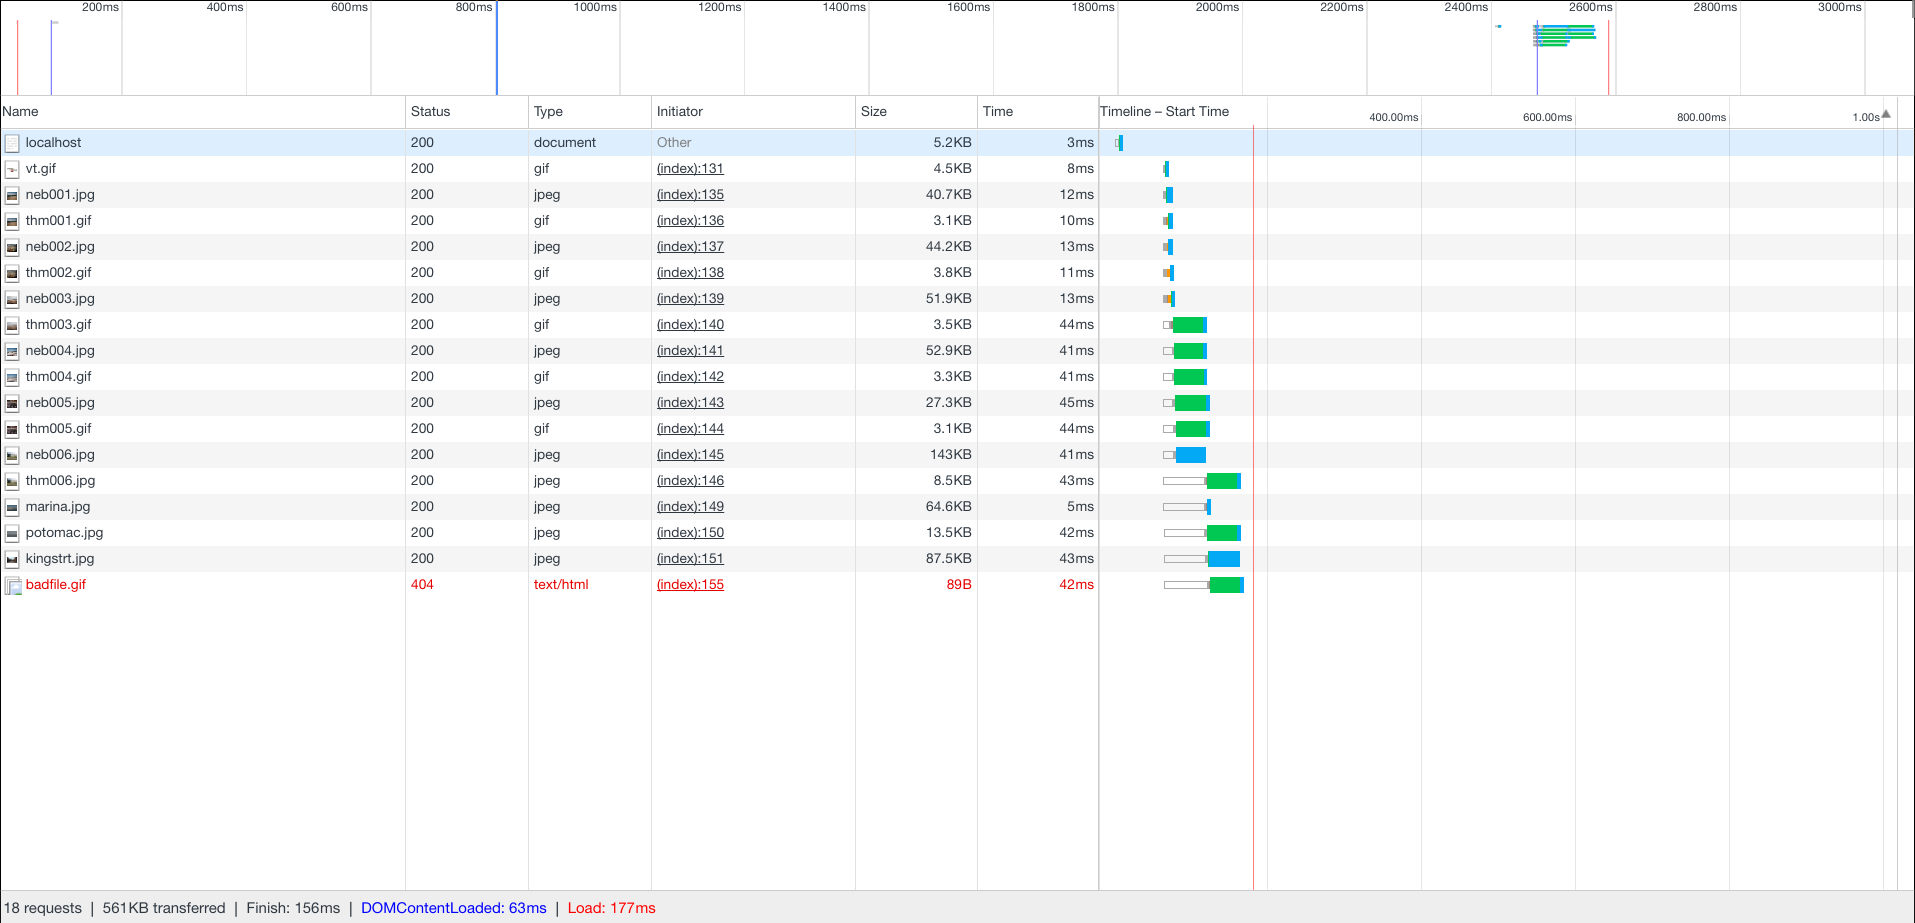
\includegraphics[width=18cm]{./multipleclients.png}


\label{orgtarget2}
\noindent Following is the condensed stderr log of opening \texttt{index.html} in firefox.

\begin{verbatim}
Connected to client 6
Request 1 from Client 5
Request 2 from Client 5
Connected to client 6
Connected to client 7
Connected to client 8
Connected to client 9
Connected to client 10
Request 1 from Client 10
Request 1 from Client 9
Request 1 from Client 8
Request 1 from Client 6
Request 1 from Client 7
Request 3 from Client 5
Request 2 from Client 8
Request 2 from Client 10
Request 2 from Client 9
Request 2 from Client 7
Request 2 from Client 6
Request 3 from Client 6
Request 4 from Client 5
Request 3 from Client 8
Request 4 from Client 6
Request 5 from Client 5
Request 5 from Client 6
Closed Client
Closed Client
Closed Client
Closed Client
Closed Client
Closed Client
\end{verbatim}

\subsection{GET Request :}
\label{sec:orgheadline11}
GET request made using Chrome

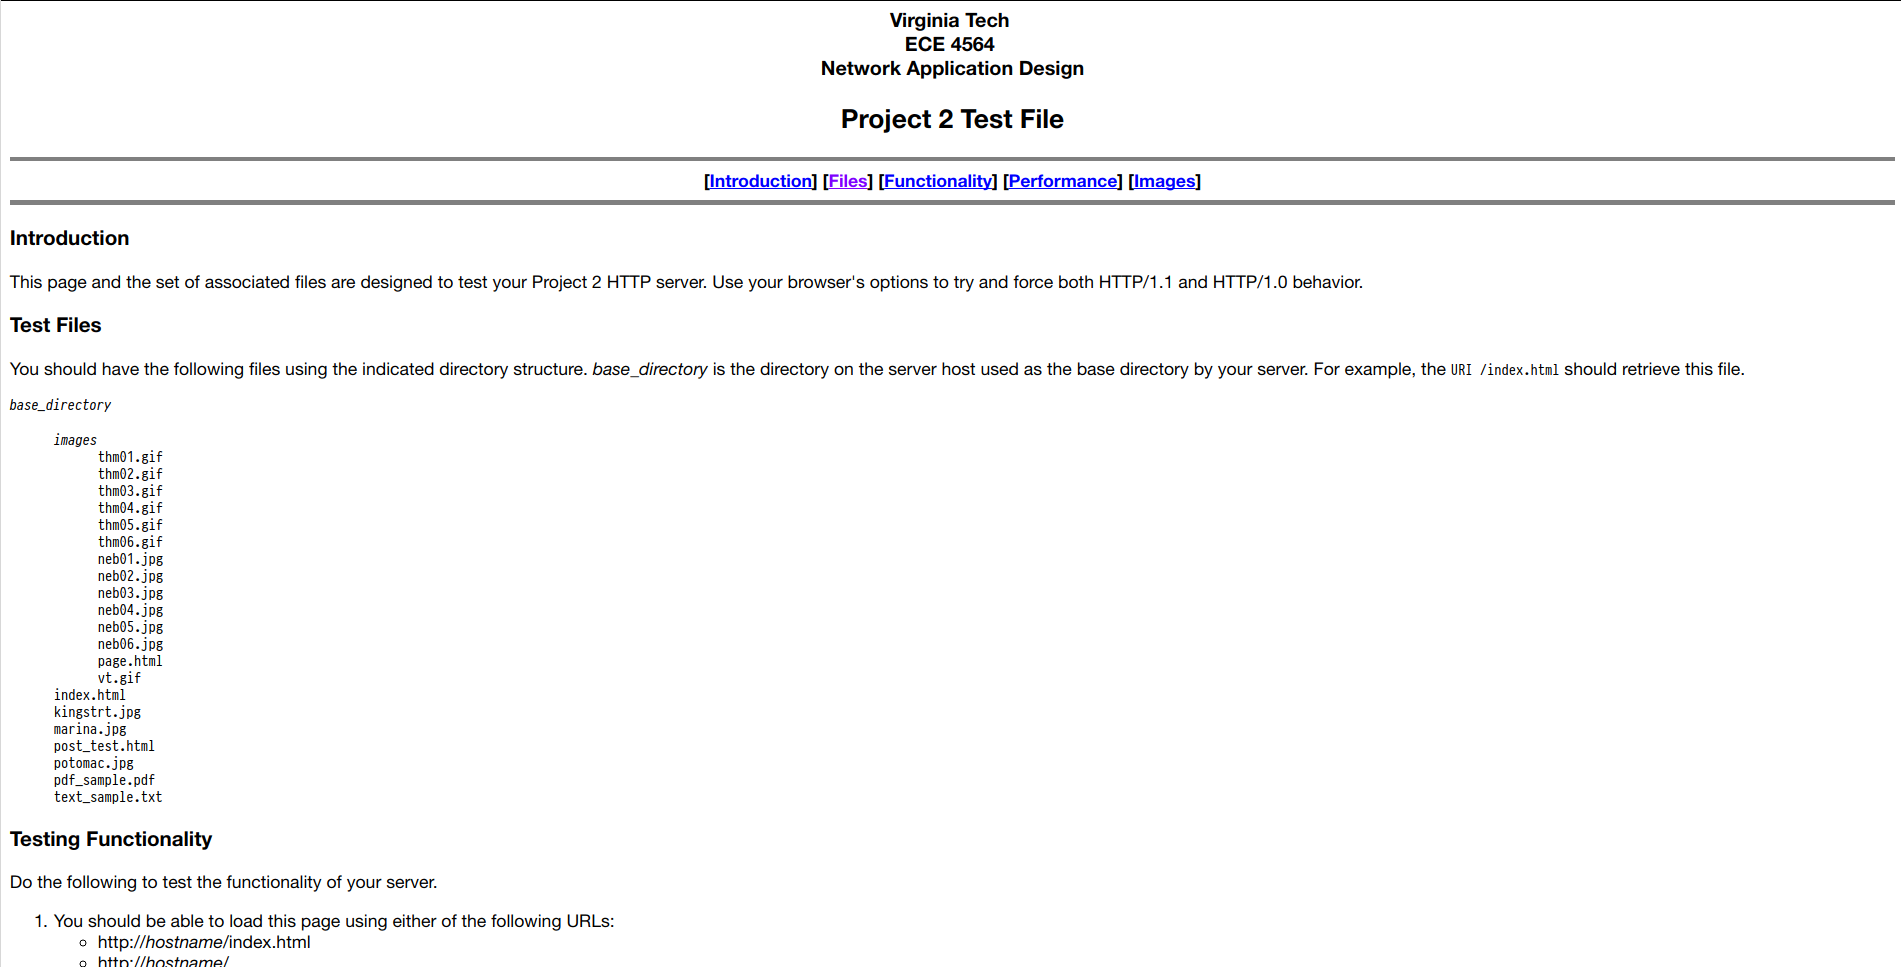
\includegraphics[width=9cm]{./index1.png}
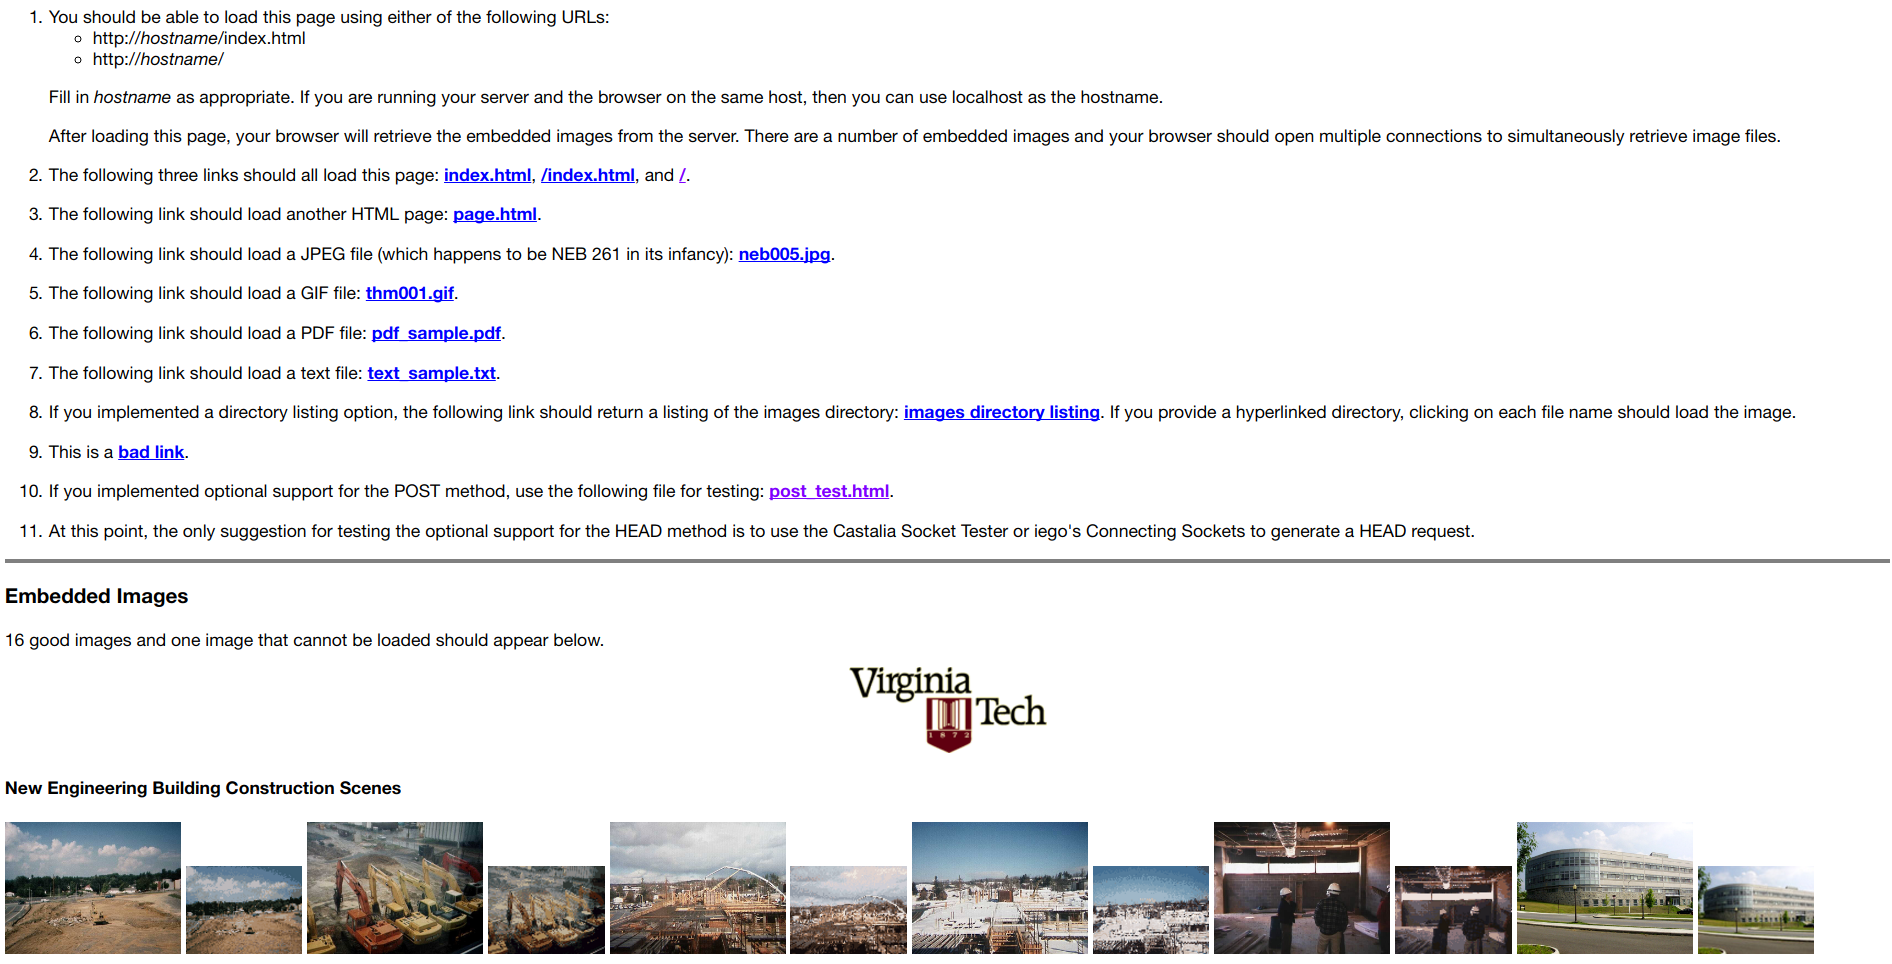
\includegraphics[width=9cm]{./index2.png} \\

\includegraphics[width=9cm]{./directorylist.png}
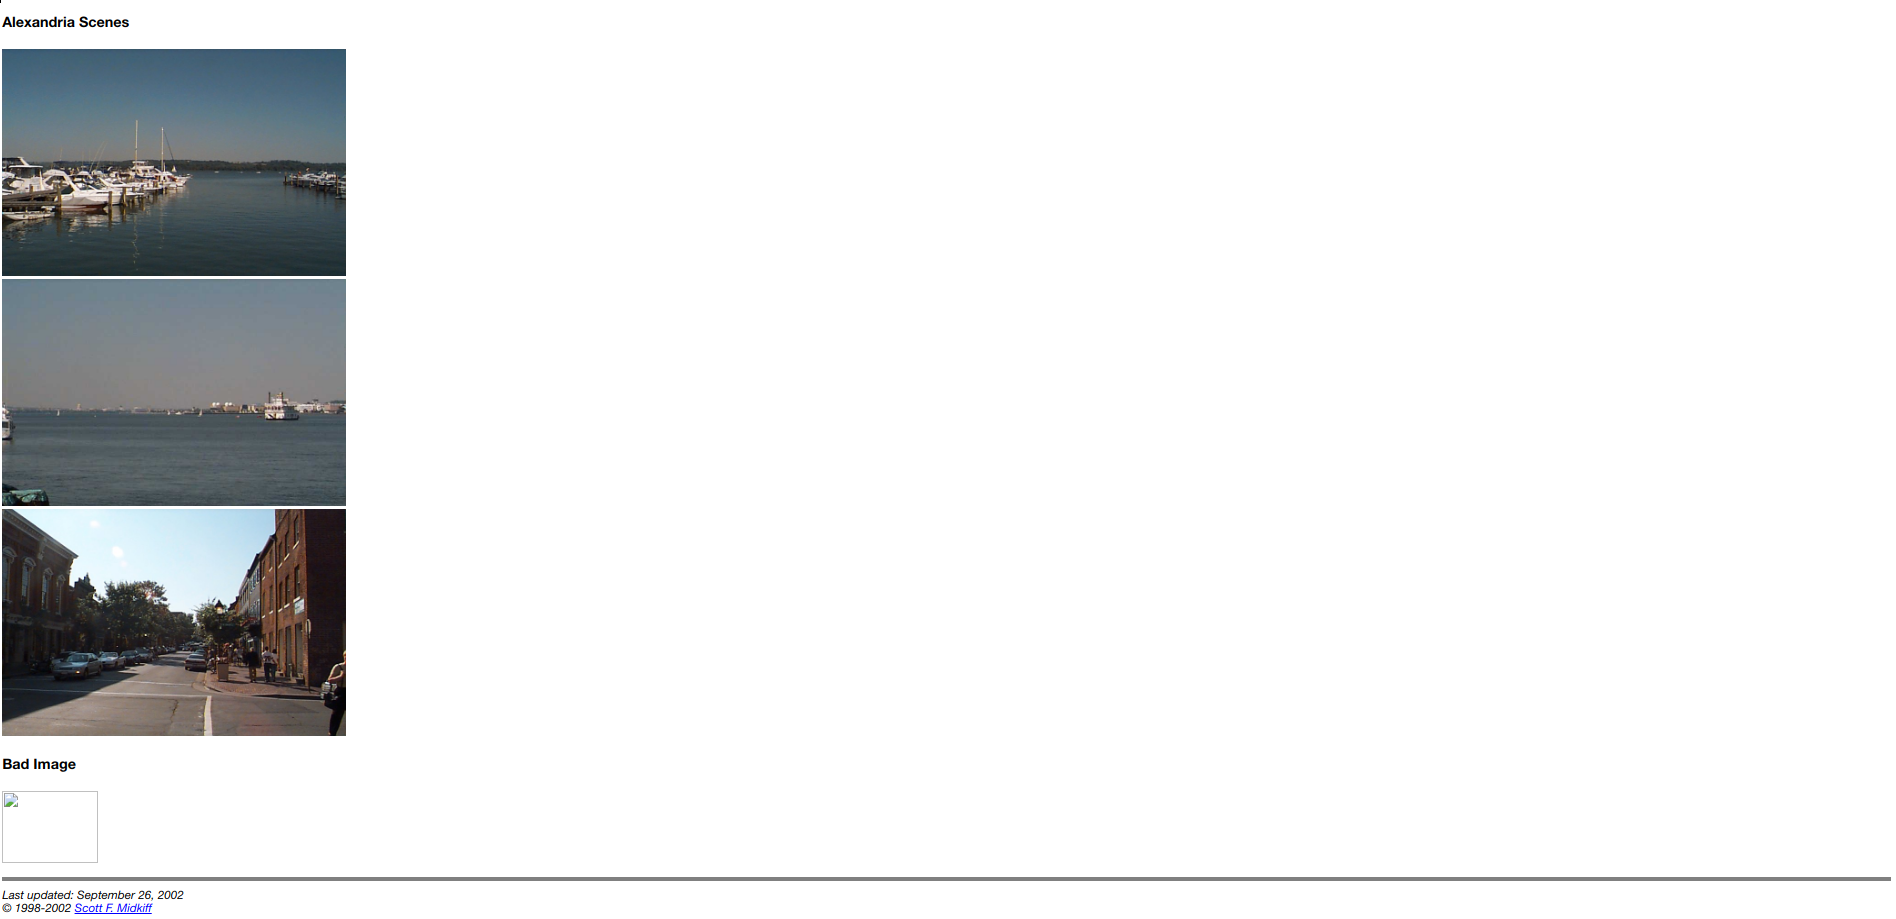
\includegraphics[width=9cm]{./index3.png}

\noindent GET request made using httpie
\begin{verbatim}
 ~/c/n/project1 $ http GET  :9577/post_test_file.txt Connection:close -v
GET /post_test_file.txt HTTP/1.1
Accept: */*
Accept-Encoding: gzip, deflate
Connection: close
Host: localhost:9577
User-Agent: HTTPie/0.9.4



HTTP/1.1 200 OK
Connection: Close
Content-Length: 93
Content-Type: text/plain
Date: Thu, 18 Aug 2016 18:52:47 GMT
Server: Alchemist

TextEntry_1=Hola&TextEntry_2=This+is+some+text+for+testing+the+POST+method.%0D%0A&Item=Item_1
\end{verbatim}

\newpage
\subsection{POST request :}
\label{sec:orgheadline15}
\label{orgtarget3}
\noindent POST Request made using httpie 

\begin{verbatim}
 ~/c/n/project1 $ base64 /dev/urandom | head -c 1000000 >! file.txt
 ~/c/n/project1 $ cat file.txt | http POST :9577/file.txt -p=Hhb
POST /file.txt HTTP/1.1
Accept: application/json
Accept-Encoding: gzip, deflate
Connection: keep-alive
Content-Length: 1000000
Content-Type: application/json
Host: localhost:9577
User-Agent: HTTPie/0.9.4

HTTP/1.1 200 OK
Content-Length: 36
Content-Type: text/html

<h1>Content written Succesfully</h1>

 ~/c/n/project1 $ diff file.txt test/file.txt
 ~/c/n/project1 $
\end{verbatim}

\subsection{HEAD request :}
\label{sec:orgheadline18}
\label{orgtarget4}
HEAD request made using httpie
\begin{verbatim}
 ~/c/n/project1 $ http HEAD  :9577/ Connection:close -v
HEAD / HTTP/1.1
Accept: */*
Accept-Encoding: gzip, deflate
Connection: close
Host: localhost:9577
User-Agent: HTTPie/0.9.4



HTTP/1.1 200 OK
Connection: Close
Content-Length: 5211
Content-Type: text/html
Date: Thu, 18 Aug 2016 18:57:32 GMT
Server: Alchemist
\end{verbatim}

\newpage
\subsection{Status Codes :}
\label{sec:orgheadline21}

Following are some of httpie requests that showcase diffrent status codes
\begin{itemize}
\item Not Implemented
\end{itemize}
\begin{verbatim}
 ~/c/n/p/doc $ http PUT  :9577/ -v
PUT / HTTP/1.1
Accept: */*
Accept-Encoding: gzip, deflate
Connection: keep-alive
Content-Length: 0
Host: localhost:9577
User-Agent: HTTPie/0.9.4

HTTP/1.0 501 Not Implemented
Connection: keep-alive
Content-Length: 29
Content-Type: text/html

<h1>501: Not Implemented</h1>
\end{verbatim}
\begin{itemize}
\item Bad Request
\end{itemize}
\begin{verbatim}
 ~/c/n/p/doc $ http PUTY  :9577/ -v
PUTY / HTTP/1.1
Accept: */*
Accept-Encoding: gzip, deflate
Connection: keep-alive
Content-Length: 0
Host: localhost:9577
User-Agent: HTTPie/0.9.4

HTTP/1.0 400 Bad Request
Connection: keep-alive
Content-Length: 25
Content-Type: text/html

<h1>400: Bad Request</h1>
\end{verbatim}
\begin{itemize}
\item Not Found
\end{itemize}
\begin{verbatim}
 ~/c/n/p/doc $ http GET  :9577/fdajlkdasj -v
GET /fdajlkdasj HTTP/1.1
Accept: */*
Accept-Encoding: gzip, deflate
Connection: keep-alive
Host: localhost:9577
User-Agent: HTTPie/0.9.4

HTTP/1.0 404 Not Found
Connection: keep-alive
Content-Length: 23
Content-Type: text/html

<h1>404: Not Found</h1>
\end{verbatim}

\subsection{Source code :}
\label{sec:orgheadline25}
\begin{verbatim}
C++ code goes here.
\end{verbatim}
\end{document}